% Indicate the main file. Must go at the beginning of the file.
% !TEX root = ../main.tex

%%%%%%%%%%%%%%%%%%%%%%%%%%%%%%%%%%%%%%%%%%%%%%%%%%%%%%%%%%%%%%%%%%%%%%%%%%%%%%%%
% 04_results
%%%%%%%%%%%%%%%%%%%%%%%%%%%%%%%%%%%%%%%%%%%%%%%%%%%%%%%%%%%%%%%%%%%%%%%%%%%%%%%%

\section{Results}
\label{results}

    \subsection{Detection}

    - after detection how many sequences are excluded

    - how many images are left per label

    \subsection{Classification Performance}

    - Table with all the models and their performance (Balanced Accuracy for the image and sequence level)

    - what models still to test? Does it make sense to do the not pretrained versions?

    \begin{figure}[ht]
    \centering
    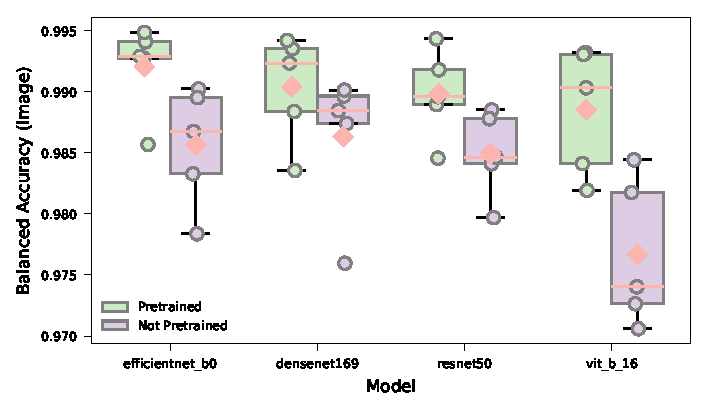
\includegraphics{figures/bal_acc_img.pdf}
    \caption{Balanced accuracy per model on the image level.}
    \label{fig:bal_acc_img}
    \end{figure}

    \subsection{Best Model}

    - More information on the best model including CM